%%%%%%%%%%%%%%%%%%%%%%%%%%%%%%%%%%%%%%%%%%%%%%%%%%%%%%%%%%%%%%%%%%%%%%%%%%%%%%%%
%2345678901234567890123456789012345678901234567890123456789012345678901234567890
%        1         2         3         4         5         6         7         8

\documentclass[letterpaper, 10 pt, conference]{ieeeconf}  % Comment this line out
                                                          % if you need a4paper
%\documentclass[a4paper, 10pt, conference]{ieeeconf}      % Use this line for a4
                                                          % paper

\IEEEoverridecommandlockouts                              % This command is only
                                                          % needed if you want to
                                                          % use the \thanks command
\overrideIEEEmargins
% See the \addtolength command later in the file to balance the column lengths
% on the last page of the document



% The following packages can be found on http:\\www.ctan.org
\usepackage{graphics} % for pdf, bitmapped graphics files
\usepackage{graphicx}
\usepackage{subcaption}
\usepackage{pgfplots}
\usepackage{array}
\usepackage{tabu}
\captionsetup{compatibility=false}
%\usepackage{epsfig} % for postscript graphics files
%\usepackage{mathptmx} % assumes new font selection scheme installed
%\usepackage{times} % assumes new font selection scheme installed
%\usepackage{amsmath} % assumes amsmath package installed
%\usepackage{amssymb}  % assumes amsmath package installed

\title{\LARGE \bf
Statistical Analysis for Identity Risk, Exposure
and Cost Using the Ecosystem of Identity Attributes
}

%\author{ \parbox{3 in}{\centering Huibert Kwakernaak*
%         \thanks{*Use the $\backslash$thanks command to put information here}\\
%         Faculty of Electrical Engineering, Mathematics and Computer Science\\
%         University of Twente\\
%         7500 AE Enschede, The Netherlands\\
%         {\tt\small h.kwakernaak@autsubmit.com}}
%         \hspace*{ 0.5 in}
%         \parbox{3 in}{ \centering Pradeep Misra**
%         \thanks{**The footnote marks may be inserted manually}\\
%        Department of Electrical Engineering \\
%         Wright State University\\
%         Dayton, OH 45435, USA\\
%         {\tt\small pmisra@cs.wright.edu}}
%}

\author{Chia-Ju Chen$^{1}$, K. Suzanne Barber and Razieh Nokhbeh Zaeem $^{2}$%} <-this % stops a space
% \thanks{*This work was not supported by any organization}% <-this % stops a space
% \thanks{$^{1}$H. Kwakernaak is with Faculty of Electrical Engineering, Mathematics and Computer Science,
%         University of Twente, 7500 AE Enschede, The Netherlands
%         {\tt\small h.kwakernaak at papercept.net}}%
% \thanks{$^{2}$P. Misra is with the Department of Electrical Engineering, Wright State University,
%         Dayton, OH 45435, USA
%         {\tt\small p.misra at ieee.org}}%
% }


\begin{document}



\maketitle
\thispagestyle{empty}
\pagestyle{empty}


%%%%%%%%%%%%%%%%%%%%%%%%%%%%%%%%%%%%%%%%%%%%%%%%%%%%%%%%%%%%%%%%%%%%%%%%%%%%%%%%
\begin{abstract}

for abstraction

\end{abstract}


%%%%%%%%%%%%%%%%%%%%%%%%%%%%%%%%%%%%%%%%%%%%%%%%%%%%%%%%%%%%%%%%%%%%%%%%%%%%%%%%
\section{INTRODUCTION}

(What are PII, identity, and identity theft)
 Personally identifiable information (PII) is any data that could potentially be used to recognize a particular person, and it's commonly used in both physical and cybersecurity field to perform personal authentication. Identity theft implies a fradulent acquisition and usage without permission of a person's PII. Modern authentication process usually requires collection of PIIs and increase the risk of exposure to identity theft and fraud criminals.

(Why is identity theft important) In 2017, the number of identity fraud victims increased by 8\% rising to 16.7 million U.S. consumers. Fraudsters stole from 1.3 million more victims in 2017 stealing 16.8 billion from U.S. consumers. More intelligent and comprehensive approach should be provided to thwart the collection of identity attributes to be compromised. 

(How can we prevent identity theft by understating the identity ecosystem)
In order to model the identity ecosystem, the initiative approach is to analyze the components from both cyber and physical aspects. Modern society introduces seamlessly merge of cyber world for both online and offline attributes. Examples of on-line attributes are one’s social media accounts, on-line shopping patterns, passwords, and email accounts. Off-line attributes are those related to the physical world such as bank accounts, credit and debit cards, Social Security Number, and one’s physical characteristics. We can further classify every attribute in person, device, organization categories.

(How do we model identity ecosystem)
The UT CID Identity Ecosystem developed at the Center for Identity (CID) at the University of Texas (UT) at Austin has constructed a graph-based model of people, devices,
and organizations. It models the relation as a Bayesian Network, performs interference for possible sources of breaches and cost if the source is compromised.
It provides a framework for understanding the value, risk and mutual relationships for pairs of PIIs. Each vertex represents an attribute whereas edges in-between implies the relationship.

(Where do we get the data for identity ecosystem? ITAP)
For data source of ecosystem, The Identity Threat Assessment and Prediction (ITAP) project is leveraged. ITAP is our endeavor focused on gathering identity theft information from such news stories, structuring this information, analyzing it, and discovering trends and characteristics, which extract data from two distinct source, either from RSS feed monitoring or from Google Alert.

(How do we map the data from ITAP to the ecosystem model. [Not Sure])

(Explanation on the paper structure)
The remainder of this article is structured as follow. Section II elaborates on the importance of statistical analysis on Ecosystem tool and set of measurement to be included. Section III presents a comprehensive evaluation and takeaways from the result. Section IV includes the related work of the identity ecosystem, identity theft, and government report. Section V concludes the research and gives insights for future works.


\section{Stats Based on Ecosystem}
(More details on Ecosystem) We have designed and implemented the Identity Ecosystem at the Center for Identity at the University of Texas at Austin as a valuable tool that models identity liaison, analyzes identity frauds and breaches, and answers several questions about identity risk management. It models identity attributes in a probabilistic model, and performs Bayesian Network-based inference to determine the posterior effects on each attribute. It map the individual identity attribute as node whereas edges in-between implies various type of connection.
Each vertex includes different properties such as type of node, risk of exposure, and intrinsic monetary value. The Ecosystem Graphical User Interface (GUI) represents each color and size based on properties independently. Figure 1 shows an example visualization that the nodes are colored based on their liability value and are sized based on their risk of exposure.

\begin{figure}[h!]
  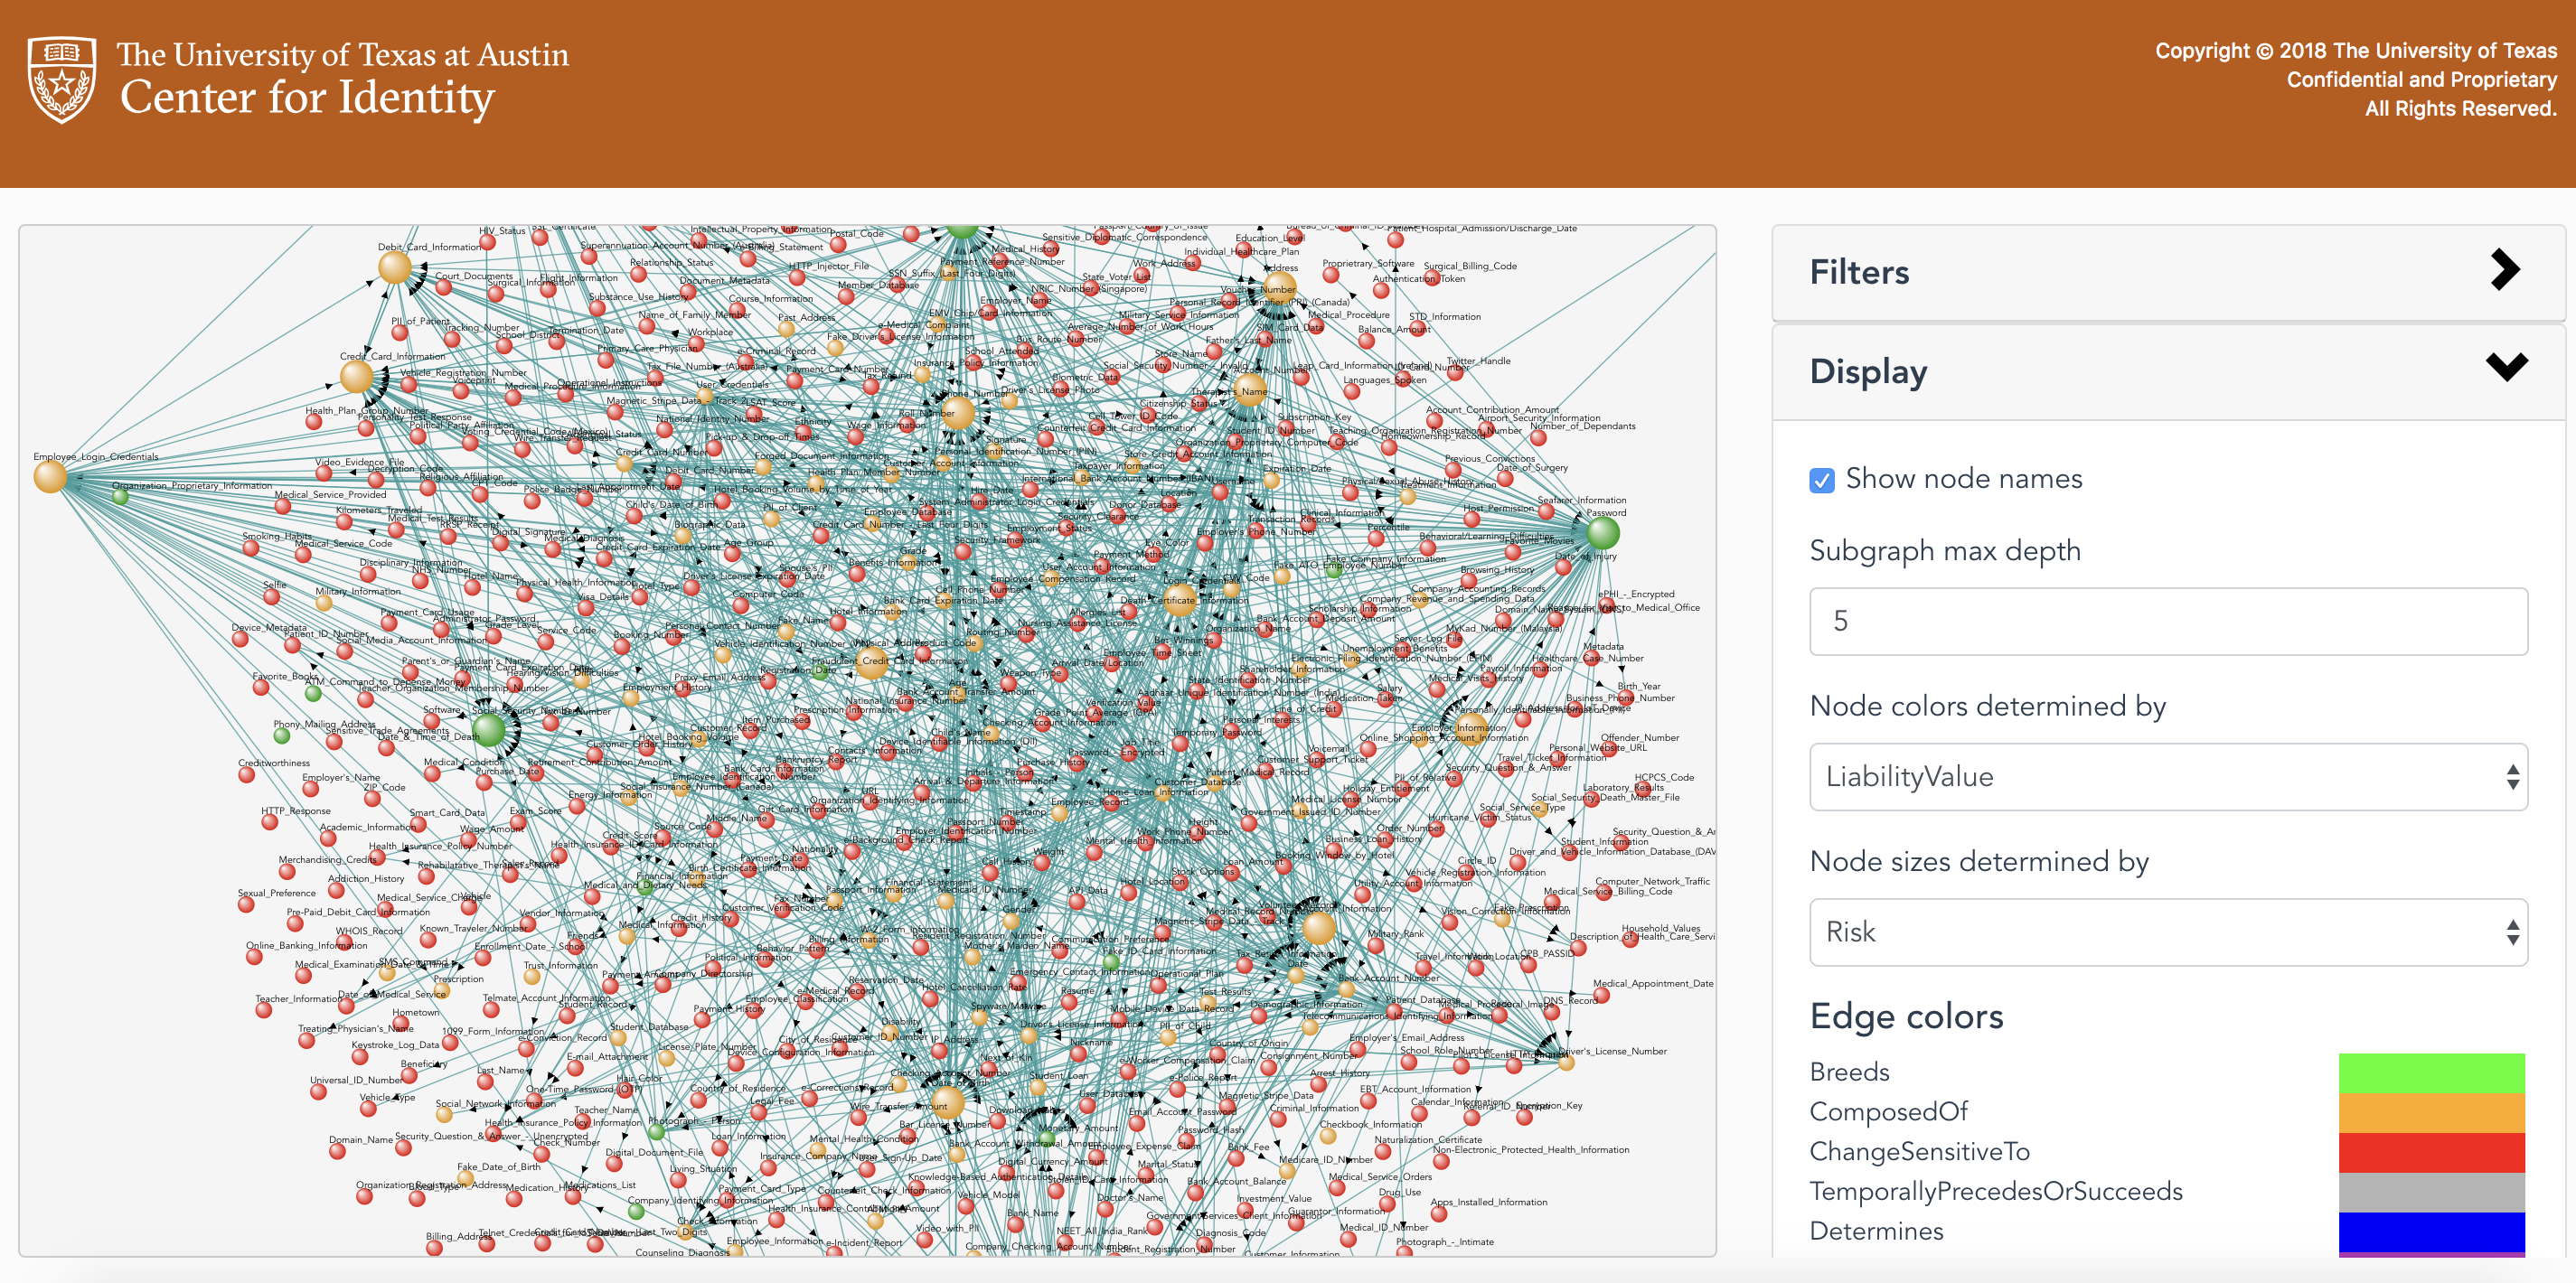
\includegraphics[width=\linewidth]{pic1.png}
  \caption{A snapshot showing Ecosystem attribute graph}
  \label{fig:pic1}
\end{figure}

(What types of stats do we consider and Why is it useful to have stats based on ecosystem)
Based on current Ecosystem framework, it can simplify the model into directed graphs with node attributes and weighted edges. We then focus on three statistical indexes on the given dataset: (1) Bar, Pie, Distribution chart based on node or edge value (2) Centrality measurement including node specific in, out-degree centrality, betweeness centrality, and closeness centrality. (3) Strongly  connected  component of nodes for identifying clusters. Based on the result, the research question we seek to answer is that "Among a graph-based network of identity, what are the underlying characteristics? Are they group as a cluster? If so, what's the isolated ones and connected ones?". We would also want to answer "Inside the network, which node is the one with most authority over the whole, meanwhile which node serves as a broadcaster for every other nodes to flow through the information?". We can further inspect possible breaches with more local attributes as in the cluster, and observe the flow inside network modeling the real-world information movement. This conclude the importance for analyzing the statistical distribution for node values and centrality measurement on Ecosystem.

\section{Statistical Charts}
We present sets of mathematical formula and statistical chart visualization in this section. The data source is from ITAP on Ecosystem, which contains 627 node attributes in total. We divide the analysis based on edge or node specific properties. We represent the Identity Ecosystem as a graph $G(V, E)$ consisting of N attributes $A_{1}$, ...,$A_{N}$ and a set of directed edges as a tuple
$e_{ij} = \langle i, j \rangle$ where $A_{i}$
is the originating node and $A_{j}$
is the target node such that $1 \leq i, j \leq N$. Each edge $e_{ij}$ represents a possible path by which $A_{j}$ can be breached given that $A_{i}$ is breached.

\subsection{Statistical charts based on edges}
We implement the pie chart to observe the percentage for nodes with/without outgoing edges or with/without incoming edges as shown in Figure 2. We can observe that a large portion of the nodes is not connected. In fact, 65\% nodes among whole are fully isolated as terms of without any inbound or outbound connections. Only a small portion is considered to be as a breach or compromised, which are vulnerable to the theft, and should make effort to protect those. 

\begin{figure}[h!]
  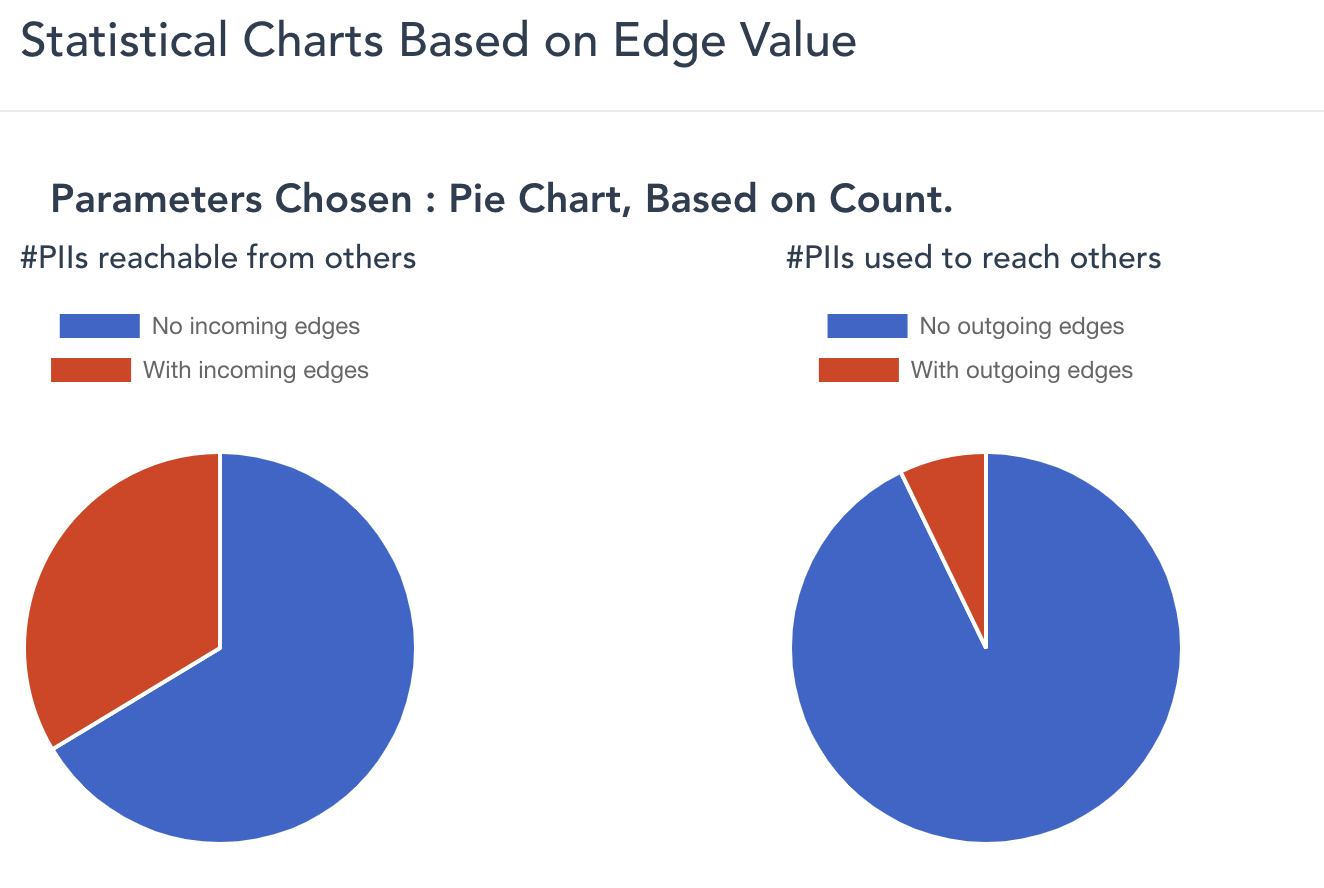
\includegraphics[width=\linewidth, height=5cm]{pic2.png}
  \caption{A snapshot showing Pie chart for percentage of nodes with/without in/out degree}
  \label{fig:pic2}
\end{figure}

%  The degree centrality of node i is defined as $Centrality^{Degree}_{i} = \sum_{j = 1}^{n} e_{ij}$ if there exist a edge from $A_{j}$ to $A_{i}$. 
Furthermore, we inspect the nodes with both in, out degree centrality measurement. Degree centrality equals the number of ties that a vertex has with other vertices. The equation for this measure is as follows, where $d(v_{i})$is the degree of $v_{i}$: 

\begin{equation}
C_{D} = d(v_{i})
\label{P}
\end{equation}

How many direct, ‘one hop’ connections each node has to other nodes within the network. From the result, it could be used to find very connected individuals, popular individuals, individuals who are likely to hold most information or individuals who can quickly connect with the wider network. 

As shown in Figure 3. It presents the top 10 PIIs in descending order with count amount. We could conclude that the attributes most likely to being acquired are Name, Credit Card Information, Date of Birth. Also, the attributes most tended to spread across the network are Customer Database, Password, Email address. Also in Figure 4, It presents the top 10 PIIs in descending order with a sum of weight on the edges, which yields the result for Name, Address, SSN for most possible compromised attributes, while Customer Database, Patient Database, User Credential are widely spread.

\begin{figure}[h!]
  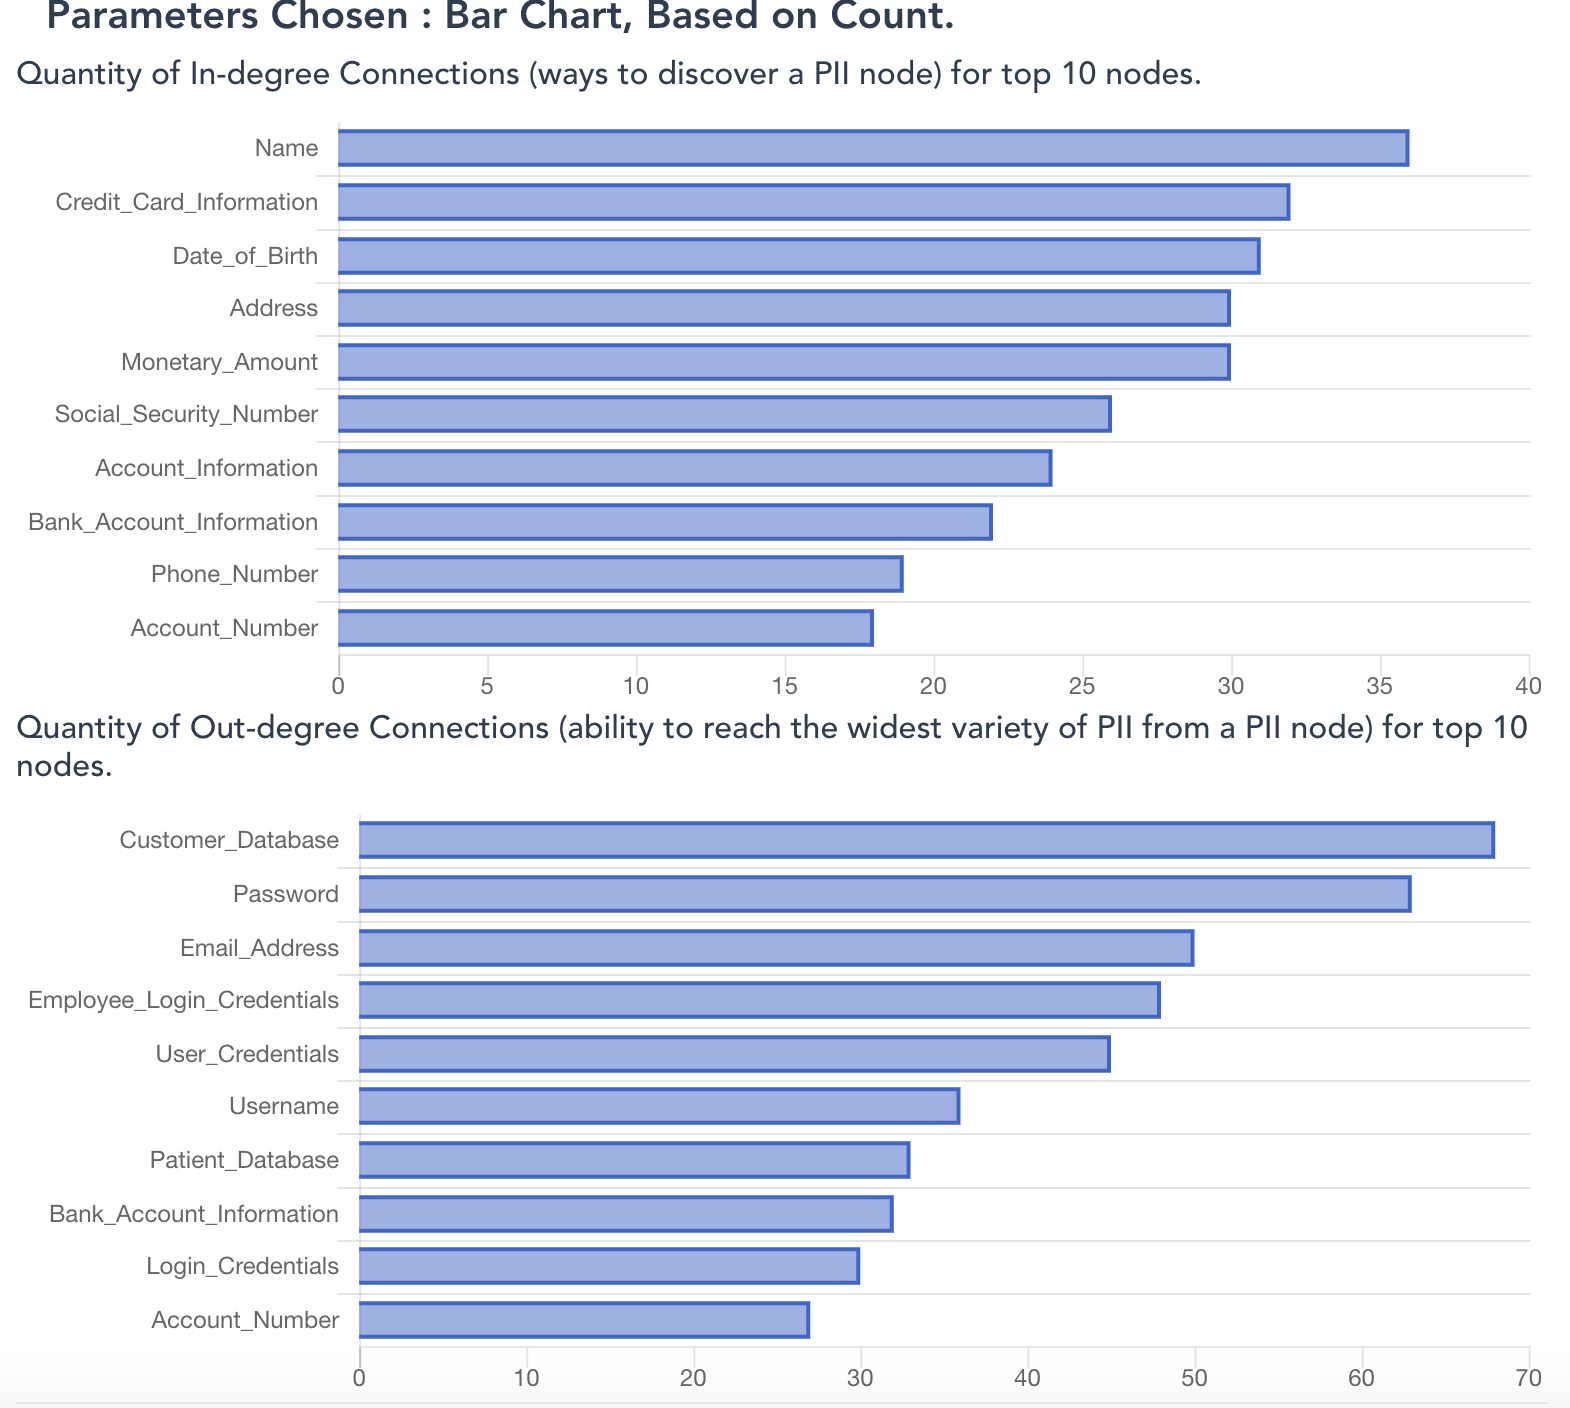
\includegraphics[width=\linewidth, height=6cm]{pic3.png}
  \caption{A snapshot showing top 10 PIIS with most in, out degree count amount}
  \label{fig:pic2}
\end{figure}

\begin{figure}[h!]
  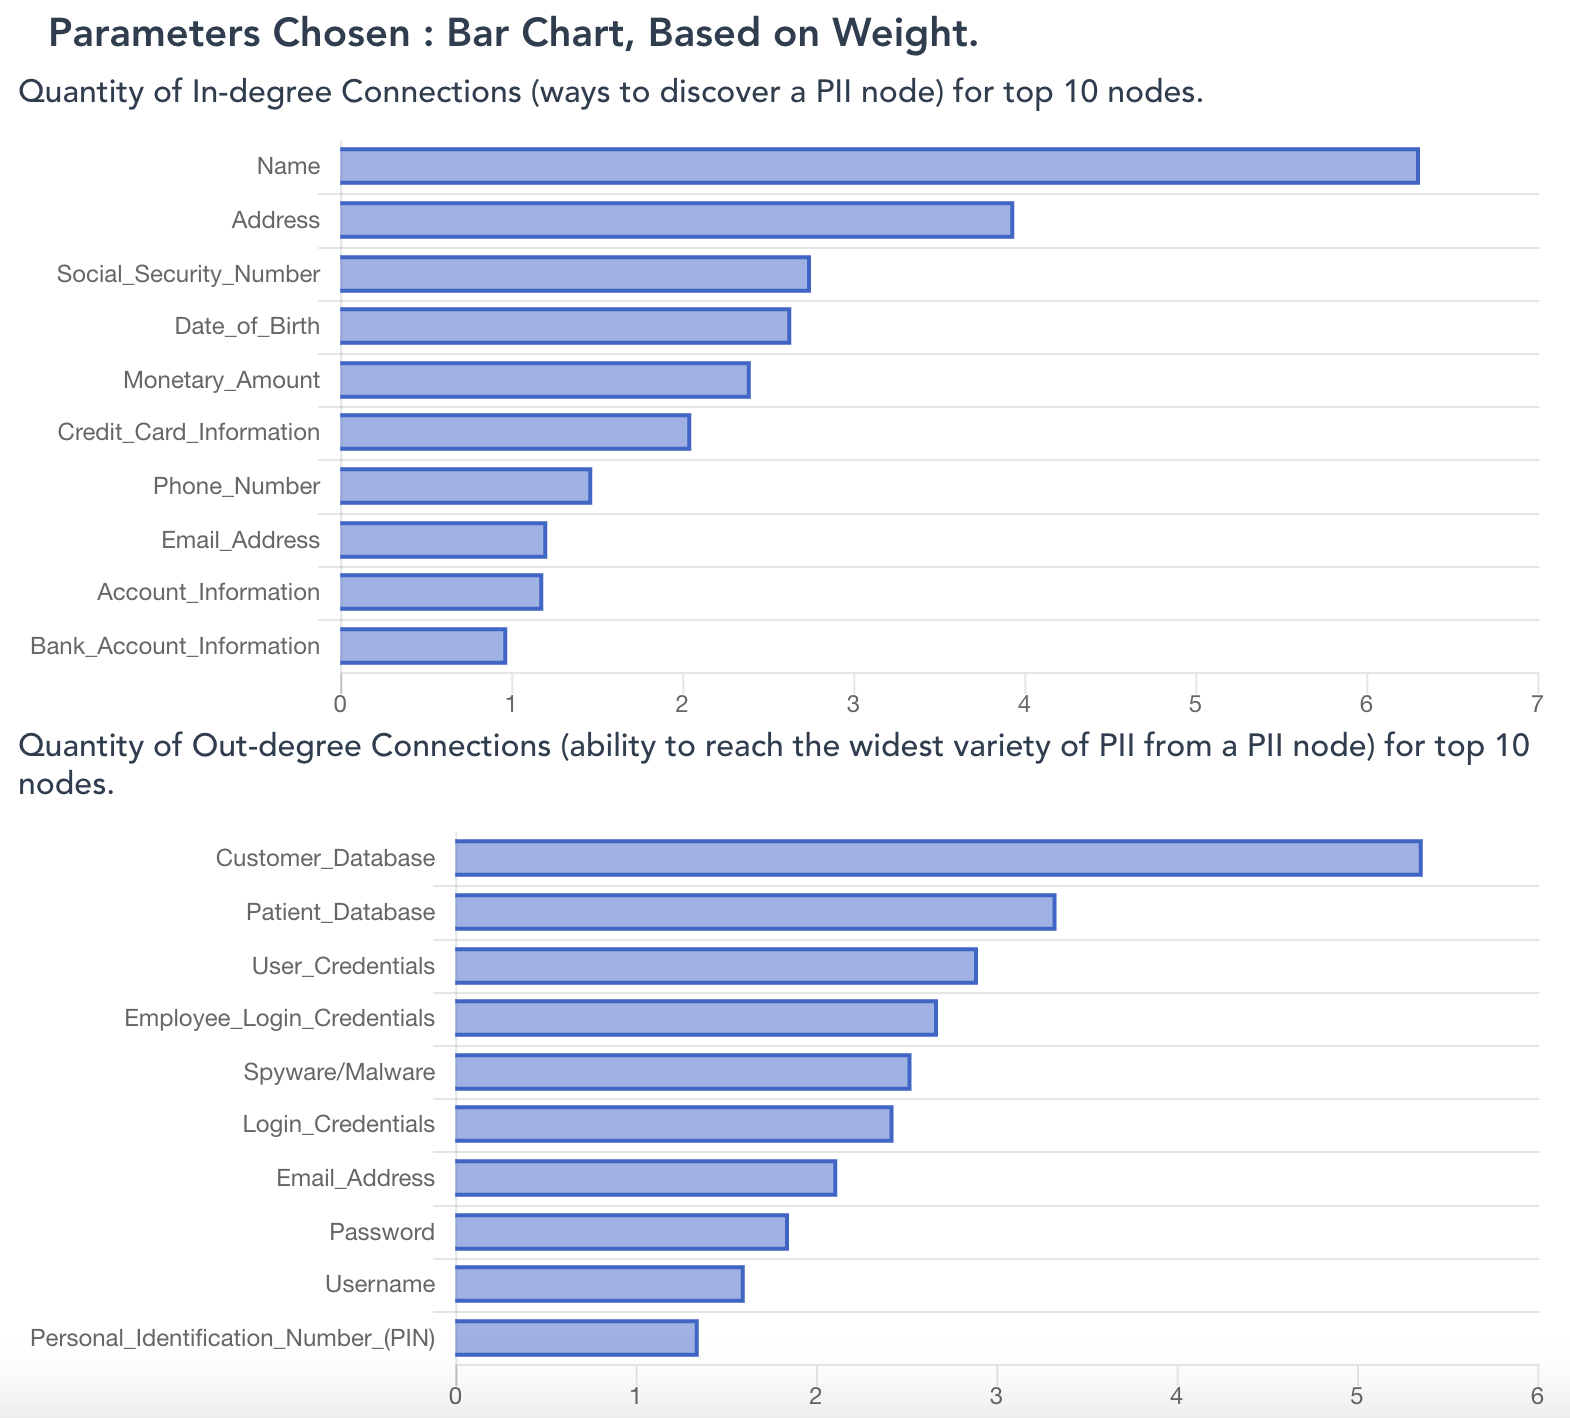
\includegraphics[width=\linewidth, height=6cm]{pic4.png}
  \caption{A snapshot showing top 10 PIIS with most in, out sum on edges}
  \label{fig:pic2}
\end{figure}

\subsection{Statistical charts based on nodes}
\begin{itemize}
\item Distribution Chart based on node risk and value
\end{itemize}

We calculate the distribution based on risk and value on each attributes to better inspect the how the underlying trend for all properties. Figure 5 gives a snapshot for distribution chart for node value with interval size 1000,00 and  Figure 6 for node risk with size 0.001.

\begin{figure}[h!]
  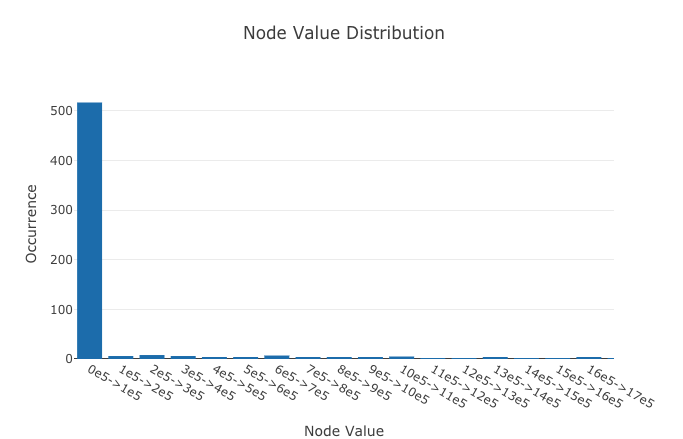
\includegraphics[width=\linewidth, height=6cm]{node_value_distribution.png}
  \caption{Distribution chart based on node value with interval size as 1000,00}
  \label{fig:node_value_distribution}
\end{figure}

\begin{figure}[h!]
  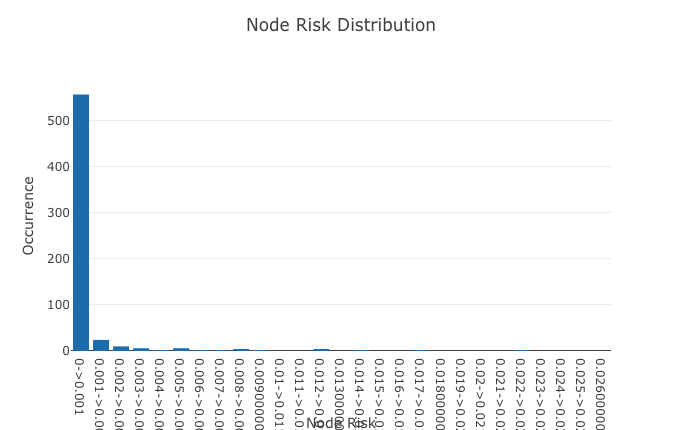
\includegraphics[width=\linewidth, height=6cm]{node_risk_distribution.png}
  \caption{Distribution chart based on node risk with interval size as 0.001}
  \label{fig:node_risk_distribution}
\end{figure}

\begin{itemize}
\item Scatter plot on Closeness v.s. Betweenness Centrality
\end{itemize}

Freeman (Cite) developed a set of measures for centrality based on betweenness. Later on Freeman (Cite) proposed four core criteras, which developed into degree, closeness, betweenness , and eigenvector centrality. We further leverage the concept of closeness and betweenness centrality to investigate Ecosystem graph.

\textbf{Closeness Centrality}
 It emphasize how close a vertex is to all other vertices in the topology -- the distance of a vertex to all others in the network by focusing on the geodesic measurement from each vertex to all others. To be more specific, it calculates the shortest path between all nodes and assigns each node a score based on its sum of shortest paths. According to Yin et al. (Cite), closeness is a evaluation for "how long it will take information to spread from a given vertex to others in the network" (Cite), which help find the individuals who are best placed to reach or be reached, and thus influence the entire network most efficiently. Also according to Freidkin(Cite), it represents the independence in the sense that they do not need to seek information from other more peripheral actors.
This yields the equation as follows, $C_{c}(v_{i})$ stands for the closeness centrality based on vertex $i$ and $shortest(v_{i},v_{j})$ is the shortest path between two vertices:
\begin{equation}
C_{c}(v_{i}) = \sum_{j = 1}^{n} \frac{1}{shortest(v_{i}, v_{j})}
\label{C}
\end{equation}

\textbf{Betweenness Centrality}
Betweenness centrality serves as an alternative concept of centrality focusing on control over the connections between other pairs of vertices. It does this by identifying all the shortest paths and then aggregating how many times each node lies on one. Denoted by $\alpha (i, j)$ the number of different shortest $\langle i, j \rangle$ paths, and by $\alpha (i, u, j)$ indicates how many times the shortest path flow through $v$, which means paths containing vertex $u$ as the inner node that $ u \neq i, j$. This gives the equation as below:
\begin{equation}
C_{B}(u) = \sum_{i \neq j \neq u}^{} \frac{\alpha (i, u, j) }{\alpha (i, j)}
\label{C}
\end{equation}

Betweenness centrality recognizes nodes who act as 'bridges' among whole and assessing the individuals who determine the flow around a system. Betweenness serves as a powerful characteristic for communication dynamics -- a high betweenness index could imply someone regulates collaboration in-between, holds authority over, disparates clusters; or infers possibly locates on the periphery of diverse clusters.

Following the centrality concept mentioned above, we calculate and introduce the scatter plot of x-axis revealing betweenness whereas y-axis for closeness indexes.  It could further be splitted into four quadrants based on combination of high, low values and on x, y axis. Denote betweeness for authority(A) and closeness for broadcaster(B), figure 5 shows the graph with blue dots represent high A and high B, orange for low A and low B, green for low A and High B, finally red as High A and low B. We can infer from the graph that most of the data points aggregate on third quadrant, and there are only several sparse distribution on points with both high betweeness and closeness centrality. It then serves as a our concern for analysis -- the attributes hold high authority and act as broadcasters in the network. If evaluated using Ecosystem model, these could be asserted as attributes that will rapidly jeopardize the remaining sub-network if already exposed, and fluctuate, boost the information flow inside the system efficiently.

\begin{figure}[h!]
  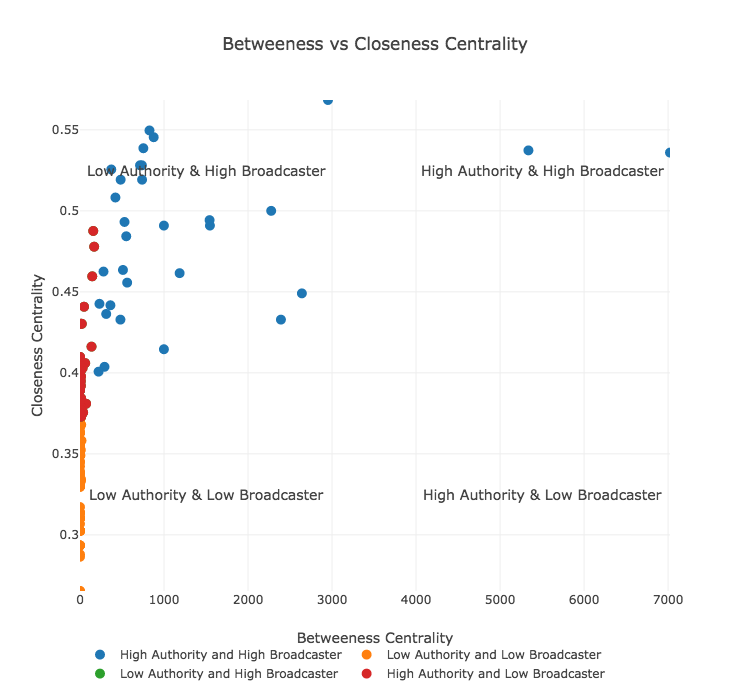
\includegraphics[width=\linewidth, height=6cm]{scatterplot.png}
  \caption{Scatter plot with x-axis showing betweeness and y-axis for closeness centrality}
  \label{fig:pic2}
\end{figure}

Furthermore, we extract top 10 elements with highest closeness centrality as Figure 8 and betweeness as Figure 9.

% top 10 closeness and top 10 betweeness bar plot

% \pgfplotstableread[row sep=\\,col sep=&]{
%     interval & closeness \\
%     Email_Address & 0.56 \\
%     Name & 0.54 \\
%     Address & 0.54 \\
%     Date_of_Birth & 0.53 \\
%     Password & 0.53 \\
%     Customer_Database & 0.53 \\
%     Phone_Number & 0.52 \\
%     Login_Credentials & 0.52 \
%     Social_Security_Number & 0.52 \\
%     Account_Information & 0.51 \\
% }\mydata
% \begin{tikzpicture}
%     \begin{axis}[
%             ybar,
%             symbolic x coords={Email_Address, Name, Address, Date_of_Birth, Password, Customer_Database, Phone_Number, Login_Credentials, Social_Security_Number, Account_Information},
%             xtick=data,
%             nodes near coords,
%         ]
%         \addplot table[x=interval,y=closeness]{\mydata};
%         \legend{Trips}
%     \end{axis}
% \end{tikzpicture}



\subsection{Strongly Connected Component}
Based on previous knowledge, large portion of nodes are isolated. From those with connections, we further identify attributes that are mutually coupled among themselves, which we defined it as a 'cluster'. Clusters serve as subsets that are dangerous source for breaches, can quickly jeopardize other members in the group and confine the flow inside sub-network. 
We propose the cluster to be a Strongly Connected Component (SCC) in the graph theory. A SCC of a directed graph $G = (V, E)$ is a maximal set of vertices $U \subseteq V$ such that for every pair of vertices $u$ and $v$ in $U$, we holds for both $u \mapsto v$ and $v \mapsto u$ (Cite), where $u \mapsto v$ means there is a directed path from u to v. Tarjan's classic serial algorithm for detection of SCCs runs linearly with respect to the number of edges and uses depth-first search. We apply the Tarjan's algorithm to compute the clusters and represent the result in Table 1. 

\begin{table}[h!]
\centering
\begin{tabu} to 0.45\textwidth { | X[l] | X[l] | X[l] | }
 \hline
    Address & Account-Number & Account-Information \\
    \hline
    Age & Bank-Account-Information & Bank-Account-Number \\
    \hline
    Biographic-Data & Birth-Certificate-Information & Credit-Card-Information \\
    \hline
    Credit-Card-Number & CVV-Code & Check-Information \\
    \hline
    Date-of-Birth & Debit-Card-Information & Driver's-License-Number \\
    \hline
    Driver's-License-Information & Date & Employee-Login-Credentials \\
    \hline
    Email-Address & Employee-Record & Expiration-Date \\
    \hline
    ID-Card-Information & Login-Credentials & Name \\
    \hline
    Password & Personally-Identifiable-Information-(PII) & Phone-Number \\
    \hline
    Personal-Identification-Number-(PIN) & Physical-Address & Passport-Information \\
    \hline
    Photograph---Person & Patient-Medical-Record & Routing-Number \\
    \hline
    Social-Security-Number & Username & W2-Form-Information \\
    \hline
\end{tabu}
\caption{List of attributes in SCC}
\label{table:1}
\end{table}

\section{Result}


\section{Conclusion and Future Work}
% A conclusion section is not required. Although a conclusion may review the main points of the paper, do not replicate the abstract as the conclusion. A conclusion might elaborate on the importance of the work or suggest applications and extensions. 

\addtolength{\textheight}{-12cm}   % This command serves to balance the column lengths
                                  % on the last page of the document manually. It shortens
                                  % the textheight of the last page by a suitable amount.
                                  % This command does not take effect until the next page
                                  % so it should come on the page before the last. Make
                                  % sure that you do not shorten the textheight too much.

%%%%%%%%%%%%%%%%%%%%%%%%%%%%%%%%%%%%%%%%%%%%%%%%%%%%%%%%%%%%%%%%%%%%%%%%%%%%%%%%



%%%%%%%%%%%%%%%%%%%%%%%%%%%%%%%%%%%%%%%%%%%%%%%%%%%%%%%%%%%%%%%%%%%%%%%%%%%%%%%%



%%%%%%%%%%%%%%%%%%%%%%%%%%%%%%%%%%%%%%%%%%%%%%%%%%%%%%%%%%%%%%%%%%%%%%%%%%%%%%%%
\section*{APPENDIX}

Appendixes should appear before the acknowledgment.

\section*{ACKNOWLEDGMENT}



%%%%%%%%%%%%%%%%%%%%%%%%%%%%%%%%%%%%%%%%%%%%%%%%%%%%%%%%%%%%%%%%%%%%%%%%%%%%%%%%

References are important to the reader; therefore, each citation must be complete and correct. If at all possible, references should be commonly available publications.



\begin{thebibliography}{99}

\bibitem{c1} G. O. Young, ÒSynthetic structure of industrial plastics (Book style with paper title and editor),Ó 	in Plastics, 2nd ed. vol. 3, J. Peters, Ed.  New York: McGraw-Hill, 1964, pp. 15Ð64.
\bibitem{c2} W.-K. Chen, Linear Networks and Systems (Book style).	Belmont, CA: Wadsworth, 1993, pp. 123Ð135.
\bibitem{c3} H. Poor, An Introduction to Signal Detection and Estimation.   New York: Springer-Verlag, 1985, ch. 4.
\bibitem{c4} B. Smith, ÒAn approach to graphs of linear forms (Unpublished work style),Ó unpublished.
\bibitem{c5} E. H. Miller, ÒA note on reflector arrays (Periodical styleÑAccepted for publication),Ó IEEE Trans. Antennas Propagat., to be publised.
\bibitem{c6} J. Wang, ÒFundamentals of erbium-doped fiber amplifiers arrays (Periodical styleÑSubmitted for publication),Ó IEEE J. Quantum Electron., submitted for publication.
\bibitem{c7} C. J. Kaufman, Rocky Mountain Research Lab., Boulder, CO, private communication, May 1995.
\bibitem{c8} Y. Yorozu, M. Hirano, K. Oka, and Y. Tagawa, ÒElectron spectroscopy studies on magneto-optical media and plastic substrate interfaces(Translation Journals style),Ó IEEE Transl. J. Magn.Jpn., vol. 2, Aug. 1987, pp. 740Ð741 [Dig. 9th Annu. Conf. Magnetics Japan, 1982, p. 301].
\bibitem{c9} M. Young, The Techincal Writers Handbook.  Mill Valley, CA: University Science, 1989.
\bibitem{c10} J. U. Duncombe, ÒInfrared navigationÑPart I: An assessment of feasibility (Periodical style),Ó IEEE Trans. Electron Devices, vol. ED-11, pp. 34Ð39, Jan. 1959.
\bibitem{c11} S. Chen, B. Mulgrew, and P. M. Grant, ÒA clustering technique for digital communications channel equalization using radial basis function networks,Ó IEEE Trans. Neural Networks, vol. 4, pp. 570Ð578, July 1993.
\bibitem{c12} R. W. Lucky, ÒAutomatic equalization for digital communication,Ó Bell Syst. Tech. J., vol. 44, no. 4, pp. 547Ð588, Apr. 1965.
\bibitem{c13} S. P. Bingulac, ÒOn the compatibility of adaptive controllers (Published Conference Proceedings style),Ó in Proc. 4th Annu. Allerton Conf. Circuits and Systems Theory, New York, 1994, pp. 8Ð16.
\bibitem{c14} G. R. Faulhaber, ÒDesign of service systems with priority reservation,Ó in Conf. Rec. 1995 IEEE Int. Conf. Communications, pp. 3Ð8.
\bibitem{c15} W. D. Doyle, ÒMagnetization reversal in films with biaxial anisotropy,Ó in 1987 Proc. INTERMAG Conf., pp. 2.2-1Ð2.2-6.
\bibitem{c16} G. W. Juette and L. E. Zeffanella, ÒRadio noise currents n short sections on bundle conductors (Presented Conference Paper style),Ó presented at the IEEE Summer power Meeting, Dallas, TX, June 22Ð27, 1990, Paper 90 SM 690-0 PWRS.
\bibitem{c17} J. G. Kreifeldt, ÒAn analysis of surface-detected EMG as an amplitude-modulated noise,Ó presented at the 1989 Int. Conf. Medicine and Biological Engineering, Chicago, IL.
\bibitem{c18} J. Williams, ÒNarrow-band analyzer (Thesis or Dissertation style),Ó Ph.D. dissertation, Dept. Elect. Eng., Harvard Univ., Cambridge, MA, 1993. 
\bibitem{c19} N. Kawasaki, ÒParametric study of thermal and chemical nonequilibrium nozzle flow,Ó M.S. thesis, Dept. Electron. Eng., Osaka Univ., Osaka, Japan, 1993.
\bibitem{c20} J. P. Wilkinson, ÒNonlinear resonant circuit devices (Patent style),Ó U.S. Patent 3 624 12, July 16, 1990. 






\end{thebibliography}
\end{document}
